\chapter{Distributed systems}\label{chapter:distributed-systems}


%%%%%%%%%%%%%%%%%%%%%%%%%%%%%%%%%%%%%%%%%%%%%%%%%%%%%%%%%%%%%%%%%
\section{Introduction}

A distributed system consists out of components that reside on different machines and communicate through message passing. This definition introduces three notable challenges:

\begin{enumerate}
	\item The lack of a global clock is largely resolved by coordinating actions through messages, but has its limitations.
	\item The nodes within this system may also fail independently and may even go undetected.
	\item Concurrency of operations brings another challenge as resources may be accessed simultanously, possibly introducing inconsistencies.
\end{enumerate}

Although these constraints make distributed systems complex to design, they come with significant benefits as well. The main motivation for developing and using distributed systems is resource sharing.

Middleware is the layer between architecture and application. It introduces an abstraction layer to build distributed applications, hiding the heterogeneity of the underlying architectural elements, e.g. protocols, servers, operating systems and so on. Middleware technology may be provide certain services such as distribution, security, ... \cite{Coulouris:2011:DSC:2029110}

\subsection{Chapter overview}




%%%%%%%%%%%%%%%%%%%%%%%%%%%%%%%%%%%%%%%%%%%%%%%%%%%%%%%%%%%%%%%%%
\section{Communication paradigms}

\subsection{Direct communication}





\subsection{Indirect communication}

In \cite{Coulouris:2011:DSC:2029110} \emph{indirect communication} is defined as "communication between entities in a distributed system through an intermediary with no direct coupling between sender and receiver". Uncoupling may be established in two ways:

\begin{itemize}
	\item \textbf{Space} : The sender does not (need to) know the identity of the receiver.
	\item \textbf{Time} : The sender and receiver does not (need to) exist at the same time as the receiver.
\end{itemize}

\textbf{Table} \ref{tab:indirectcommunication-uncoupling} categorizes a number of technologies according to their support for time and/or space uncoupling. Note the relationship between time uncoupling and asynchronous communication. However, in the case of strict uncoupling in time, the receiving end does not necessarily exist at the time of sending, as mentioned earlier \cite{Coulouris:2011:DSC:2029110}.


\begin{table}[h]
	\caption{Overview of space and time coupling for distributed communication paradigms.}
	\label{tab:indirectcommunication-uncoupling}
	\begin{tabular}{p{100px} | p{125px} | p{125px}}
															& \textbf{Time-coupled} 	& \textbf{Time-uncoupled} \\
		\hline
		\textbf{Space-coupled} 		& Message-passing, RMI 		&  \\
		\textbf{Space-uncoupled} 	& IP multicast						& Publish-subscribe, tuple spaces, message queues \\
		\hline
	\end{tabular}
\end{table}

Typical applications of indirect communication is in mobile environments, cloud computing, and event dissemination where receivers are unknown or change rapidly \cite{Coulouris:2011:DSC:2029110}.

Coulouris et al. distinguish between five variations of indirect communication, namely:
\begin{enumerate}
	\item Group communication;
	\item Publish-subscribe systems;
	\item Message queues;
	\item Distributed shared memory;
	\item Tuple spaces.
\end{enumerate}


\subsubsection{Group communication}

In group communication the messages within a distributed system are sent to a group, and from there sent to all other members of the group. The sender has no knowledge of the identities of the receivers, hence the indirection \cite{Coulouris:2011:DSC:2029110}. This kind of communication is called broadcasting where the sender forms a one-to-many relationship with the other members of the group.

Groups may be open or closed. In closed groups only members can multicast to it, opposed to open groups where processes outside the group can multicast to it as well.

\textbf{Figure} \ref{fig:groupcommunication} gives an overview of the basic operations of group management. The operation set for group communication is shown in \textbf{table} \ref{tab:api:groupcommunication}.


\begin{figure}
	\begin{center}
		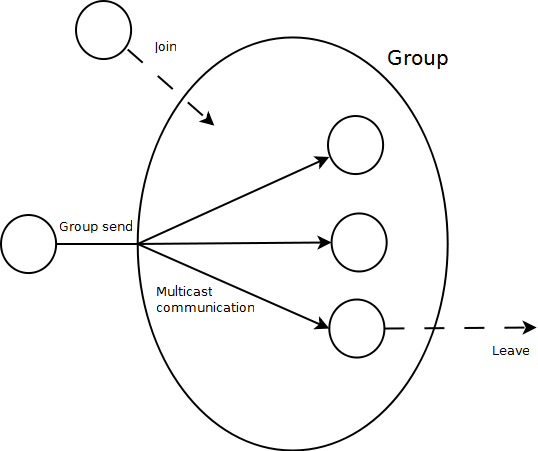
\includegraphics[width=0.5\textwidth]{img/systems-and-architectures/groupcommunication}
	\end{center}
	\caption{Group membership management in group communication.}
	\label{fig:groupcommunication}
\end{figure}

\begin{table}
	\caption{Group communication API.}
	\label{tab:api:groupcommunication}
	\begin{tabular}{p{150px} | p{250px}}
		\textbf{Operation} & \textbf{Description} \\
		\hline
		join (group) & \emph{A process joins the group.} \\
		leave (group) & \emph{A process leaves the group.} \\
		send (group, message) & \emph{Send a message to the group. The group indirection layer propagates the message to all other members.} \\
		\hline
	\end{tabular}
\end{table}


\subsubsection{Publish-subscribe systems}

A publish-subscribe system is a platform where \emph{subscribers} can subscribe to certain events provides by \emph{publishers}. The system then matches published events against subscriptions. Subscribers then receive an update if successful matches are found.

Publishers form a one-to-many relationship with their subscribers, but the publishers do not know who is subscribed. Subscribers also do not need to know the publisher, as long as they can specify which kind of messages they would like to receive . Publish-subscribe systems are uncoupled in time as they provide asynchronous communication between senders and receivers \cite{Coulouris:2011:DSC:2029110}.

The operations of a publish-subscribe system are listed in \textbf{Table} \ref{tab:api:publishsubscribersystems}.


\begin{table}[h]
	\caption{Publish-subscribe system API.}
	\label{tab:api:publishsubscribersystems}
	\begin{tabular}{p{150px} | p{250px}}
		\textbf{Operation} & \textbf{Description} \\
		\hline
		publish (event) 			& \emph{A publisher publishes an event.} \\
		subscribe (filter) 		& \emph{A subscriber subscribes to a set of events through a filter.} \\
		unsubscribe (filter) 	& \emph{A subscriber unsubscribes from a set of events.} \\
		notify (event) 				& \emph{Deliver events to its subscribers.} \\
	  advertise (filter) 		& \emph{A publisher declare the nature of the events they will produce.} \\
		unadvertise (filter) 	& \emph{A publisher revokes the advertisement.} \\
		\hline
	\end{tabular}
\end{table}



\begin{figure}[h]
	\begin{center}
		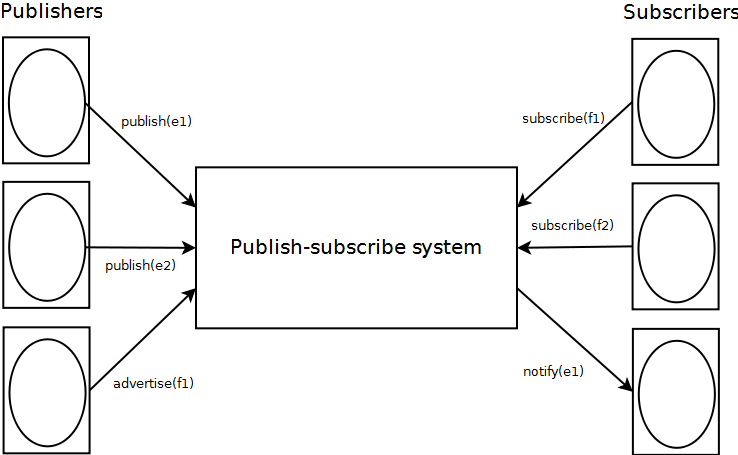
\includegraphics[width=0.6\textwidth]{img/systems-and-architectures/publish-subscribesystem}
	\end{center}
	\caption{Publish-subscribe system architecture.}
	\label{fig:publish-subscribesystem}
\end{figure}




\subsubsection{Message queues}

Message queues are a form of message-oriented middleware. A message queue introduces a layer of indirection between \emph{producers} and \emph{consumers}. A producers sends messages to a queue, next consumers receive messages from these queues. Message queues are uncoupled in time, but not in space. The relation between a consumer and a producer through a message is one-to-one \cite{Coulouris:2011:DSC:2029110}.

The operations that can be invoked on a message queue are listed in \textbf{table} \ref{tab:api:messagequeues}.


\begin{table}[h]
	\caption{Message queue API.}
	\label{tab:api:messagequeues}
	\begin{tabular}{p{150px} | p{250px}}
		\textbf{Operation} & \textbf{Description} \\
		\hline
		send (message) & \emph{A producer sends a message to the queue.} \\
		receive (message) & \emph{A blocking receive operation. The consumer will block until an appropriate message is available.} \\
		poll (message) & \emph{The consumer checks the status of the queue. A message is returned if available, else a negative signal.} \\
		notify (message) & \emph{Start listening for event notications if a message is available.} \\
		\hline
	\end{tabular}
\end{table}


Messages are usually added to the queue based on the first-in-first-out (FIFO) policy, but priorities may be used as well. Message queues try to ensure reliable delivery by persisting messages: messages are eventually delivered (time uncoupling). Messages are also only sent once and as received to provide integrity \cite{Coulouris:2011:DSC:2029110}.

The consumers may receive messages by actively checking (polling) if messages are available, or by receiving notifications that messages have become available. Messages may be filtered based on certain properties \cite{Coulouris:2011:DSC:2029110}.

\begin{figure}[h]
	\begin{center}
		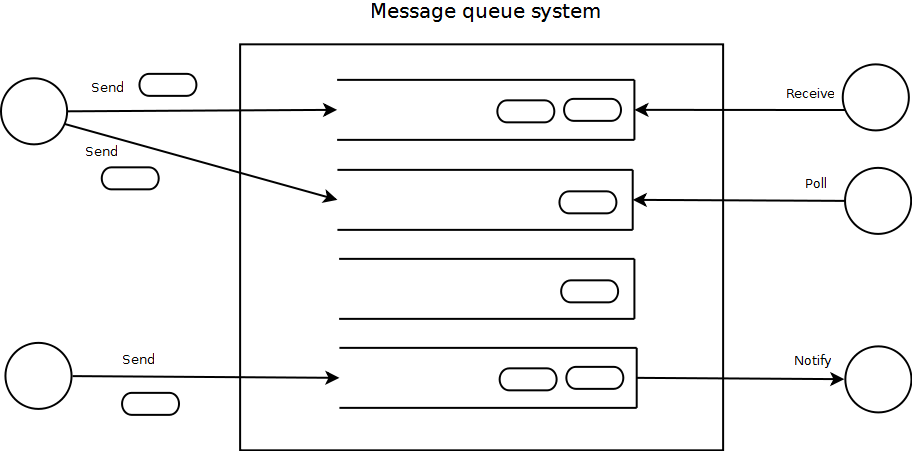
\includegraphics[width=0.7\textwidth]{img/systems-and-architectures/messagequeues}
	\end{center}
	\caption{The message queue paradigm.}
	\label{fig:messagequeues}
\end{figure}



\subsubsection{Distributed shared memory}

The objective of distributed shared memory (DSM) is to share data between computers. Each computer has a local copy of the data. This data is kept up to date by passing messages between each node over the DSM middleware. \textbf{Table} \ref{tab:api:dsm} shows the operations for DSM.

\begin{table}[h]
	\caption{Distributed shared memory API.}
	\label{tab:api:dsm}
	\begin{tabular}{p{150px} | p{250px}}
		\textbf{Operation} & \textbf{Description} \\
		\hline
		read (data) 			& \emph{Read from the shared memory.} \\
		write (data) 			& \emph{Write to the shared memory} \\
		update (message) 	& \emph{Send an update message to the other members of the distributed shared memory.} \\
		\hline
	\end{tabular}
\end{table}


\begin{figure}[h]
	\begin{center}
		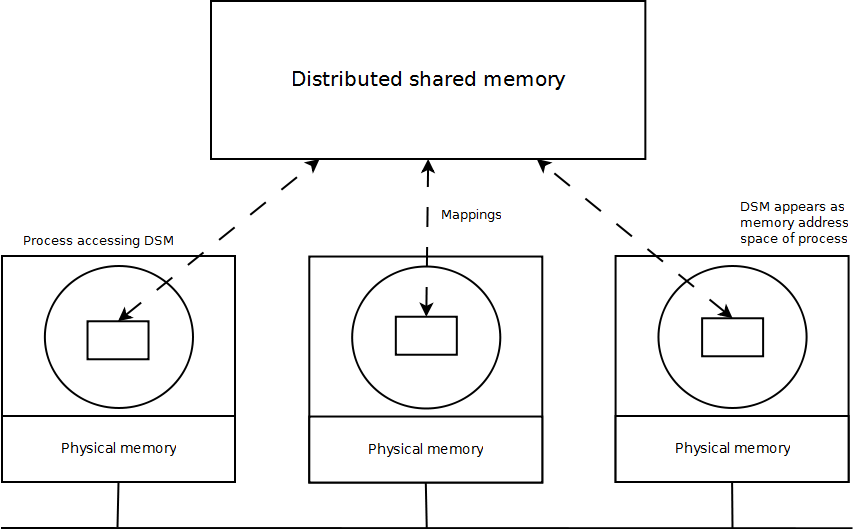
\includegraphics[width=0.6\textwidth]{img/systems-and-architectures/dsm}
	\end{center}
	\caption{Distributed shared memory architecture.}
	\label{fig:dsm}
\end{figure}



\subsubsection{Tuple spaces}

A tuple space is a form of distributed memory where "processes communicate indirectly by placing tuples in a tuple space from which other processes can read and remove them" \cite{Coulouris:2011:DSC:2029110}. Space uncoupling is achieved as the sending and receiving processes may come from anywhere. Tuples may be taken from the space at any time and may even reside indefinately in the tuple space, thus achieving time uncoupling.

A tuple is typically of the form <var1, var2>, e.g. \emph{<"hugo",1.19>}. A number of operations can be executed on a tuple space as listed in \textbf{table} \ref{tab:api:tuplespaces}.


\begin{table}[h]
	\caption{Tuple space API.}
	\label{tab:api:tuplespaces}
	\begin{tabular}{p{150px} | p{250px}}
		\textbf{Operation} & \textbf{Description} \\
		\hline
		read (tuple) 	& \emph{Reads a tuple from the tuple space.} \\
		take (tuple) 	& \emph{Extract a tuple from the tuple space.} \\
		write (tuple) & \emph{Write a new tuple to the tuple space.} \\
		\hline
	\end{tabular}
\end{table}


\begin{figure}[h]
	\begin{center}
		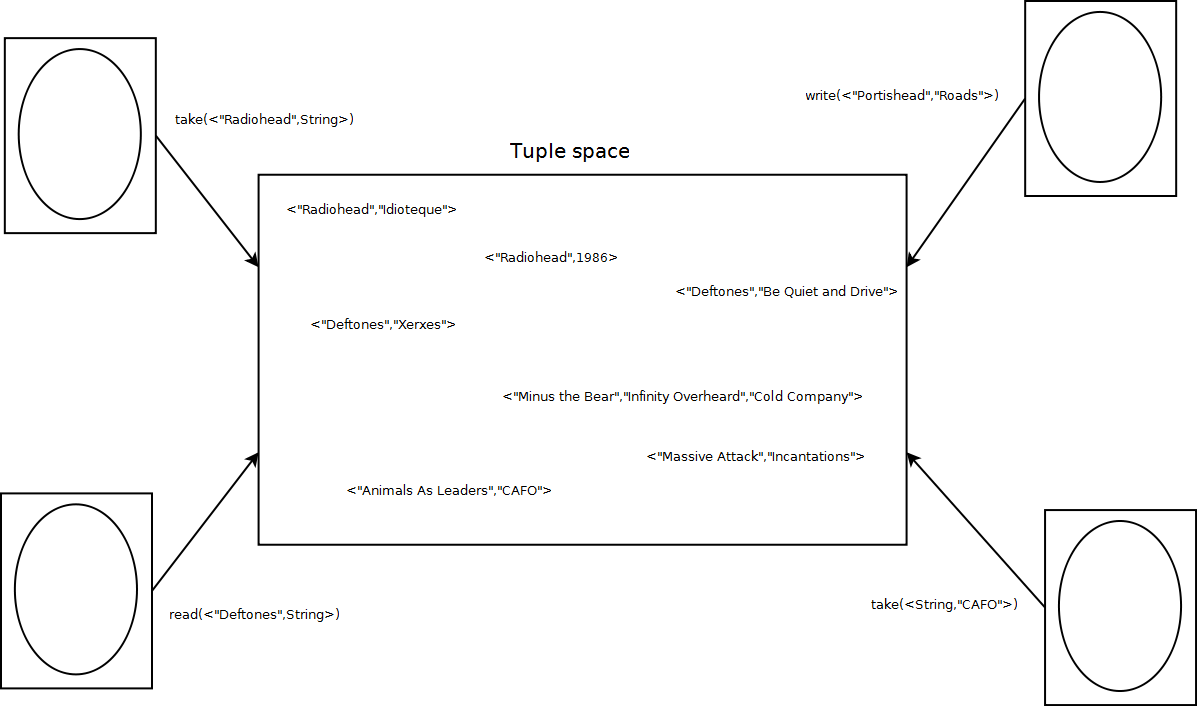
\includegraphics[width=0.6\textwidth]{img/systems-and-architectures/tuplespace}
	\end{center}
	\caption{Tuple space abstract example.}
	\label{fig:tuplespace}
\end{figure}




%%%%%%%%%%%%%%%%%%%%%%%%%%%%%%%%%%%%%%%%%%%%%%%%%%%%%%%%%%%%%%%%%
\section{Replication}

\subsection{Definitions and models}

\emph{Replication} is "the maintenance of copies of data at multiple computers" \cite{Coulouris:2011:DSC:2029110}. In the context of replication data can be thought of as \emph{objects}, where each \emph{logical} object is in fact a collection of physical copies called \emph{replicas}. \emph{Replication transparency} may be included as another requirement for distributed system design. Replication helps making distributed systems more effective in three ways \cite{Coulouris:2011:DSC:2029110}:
\begin{enumerate}
	\item \textbf{Performance enhancement} : caching at server and client side helps resolving latency problems. Replication of immutable data is trivial, whereas data that can change over time must be kept up to date. In the latter case, the generated overhead may put a limit to the performance increase.
	\item \textbf{Increased availability} : Server failures and communication disconnections may decrease availability of resources. By keeping local copies of data, the availability of this data naturally increases.
	\item \textbf{Fault tolerance} : Maintaining correctness of replicated data is imperative for the effectiveness of the replication model.
\end{enumerate}

The model sketched in \textbf{figure} \ref{fig:replicationmodel} consists out of a number of components called \emph{replica managers} and a number of clients with a component called a \emph{front end} associated with it. Replica managers apply operations directly on the replicas, often using atomic operations. In this case the state of the replicas is a deterministic function of the initial state the collection of applied operations \cite{Coulouris:2011:DSC:2029110}.

\begin{figure}[h]
	\begin{center}
		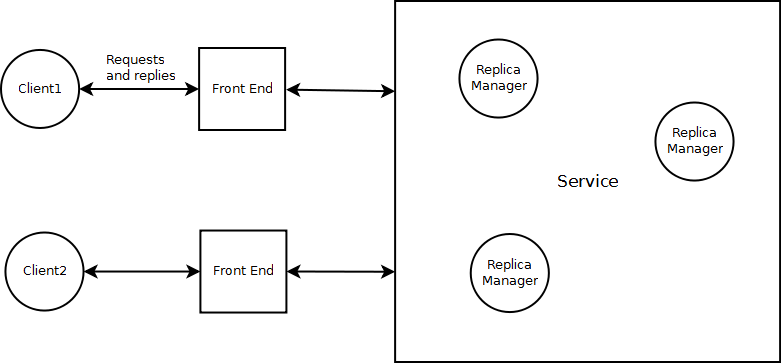
\includegraphics[width=0.7\textwidth]{img/systems-and-architectures/replicationmodel}
	\end{center}
	\caption{Basic architectural model for the management of replicated data.}
	\label{fig:replicationmodel}
\end{figure}



Replica managers provide a service, i.e. access to objects, to the clients. Clients indirectly access object through the methods listed in \textbf{table} \ref{tab:api:replica-manager}. The front end handles the client requests and uses messages to communicate with the replica managers. This abstraction layer ensures replication transparency at the client side \cite{Coulouris:2011:DSC:2029110}.


\begin{table}[h]
	\caption{Replica manager service API.}
	\label{tab:api:replica-manager}
	\begin{tabular}{p{150px} | p{250px}}
		\textbf{Operation} & \textbf{Description} \\
		\hline
		readOnlyRequest (object) & \emph{Template method for an invocation by the client on an object with no updates on the object itself.} \\
		updateRequest (object) & \emph{Template method for an invocation by the client on an object, which alteres the state of the object.} \\
		\hline
	\end{tabular}
\end{table}

Coulouris et al. \cite{Coulouris:2011:DSC:2029110} list five phases in which the request is handles by the system:
\begin{enumerate}
	\item \textbf{Request} : The front end issues a request to one or more replica managers, either through unicast or through multicast. In the first case the replica manager will propagate the message to other replica managers.
	\item \textbf{Coordination} : Replica managers decide whether or not the request can be applied, i.e. the request will not introduce inconsistencies, and how the requests will be ordered. Possible ordering policies are for example FIFO, causal or total ordering.
	\item \textbf{Execution} : The request is executed by the replica managers.
	\item \textbf{Agreement} : The replica managers decide whether or not the commit the results of the request.
	\item \textbf{Response} : One or more replica managers communicate the result to the front end.
\end{enumerate}


\subsubsection{Group views}

The size of the set of replica managers may be be constant, i.e. membership is static, or vary, i.e. membership is dynamic. To manage this kind of groups, the group communication paradigm is often applied; particularly in the case of dynamic membership where the join and leave operations are concerned \cite{Coulouris:2011:DSC:2029110}.

To manage groups, \emph{group views} are used. These are ordered lists of the current group members. Each group member has a unique process identifier. Group views are generated as members join or leave, after processes are notified of changes through view delivery. Correct view delivery requires a number of guarantees to be met \cite{Coulouris:2011:DSC:2029110}:
\begin{itemize}
	\item \textbf{Order} : If a processe delivers views v(g) and v'(g), then no other process will deliver v'(g) before v(g).
	\item \textbf{Integrity} : If a process delivers a view, then that process is part of the view.
	\item \textbf{Non-triviality} : A process q that is indefinitely reachable from a process p will always be in the views that p delivers.
\end{itemize}
In the case of \emph{view-synchronous group communication} additional constraints are to be met. \textbf{Figure} \ref{figure:viewsynchronousgroupcommunication} gives an overview of allowed and disallowed scenarios based on the following requirements \cite{Coulouris:2011:DSC:2029110}:
\begin{itemize}
	\item \textbf{Agreement} : Correct processes deliver the same sequence of views and set of messages within any given view.
	\item \textbf{Integrity} : If a correct process delivers a message m, this process will not deliver m again.
	\item \textbf{Validity} : Correct processes always deliver the messages that they send.
\end{itemize}



\begin{figure}[h]
        \centering
        \begin{subfigure}[t]{0.4\textwidth}
                                        \centering
                                        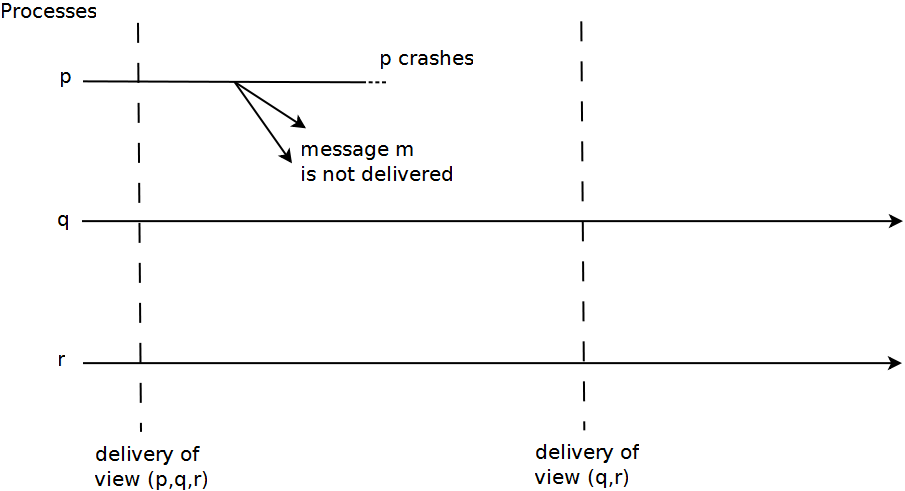
\includegraphics[width=\textwidth]{img/systems-and-architectures/viewsynchronousgroupcommunication_a}
                                        \caption{Allowed case where the messages are not delivered and process p crashes.}
                                        \label{figure:viewsynchronousgroupcommunication:a}
        \end{subfigure}%
        ~
        \begin{subfigure}[t]{0.4\textwidth}
                                        \centering
                                        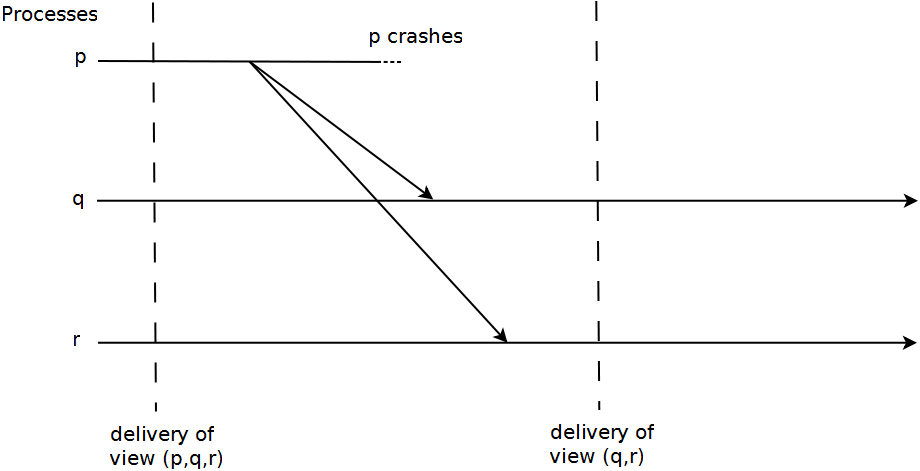
\includegraphics[width=\textwidth]{img/systems-and-architectures/viewsynchronousgroupcommunication_b}
                                        \caption{Allowed case where the messages are delivered before the delivery of view (q,r).}
                                        \label{figure:viewsynchronousgroupcommunication:b}
        \end{subfigure}
        ~
        \begin{subfigure}[t]{0.4\textwidth}
                                        \centering
                                        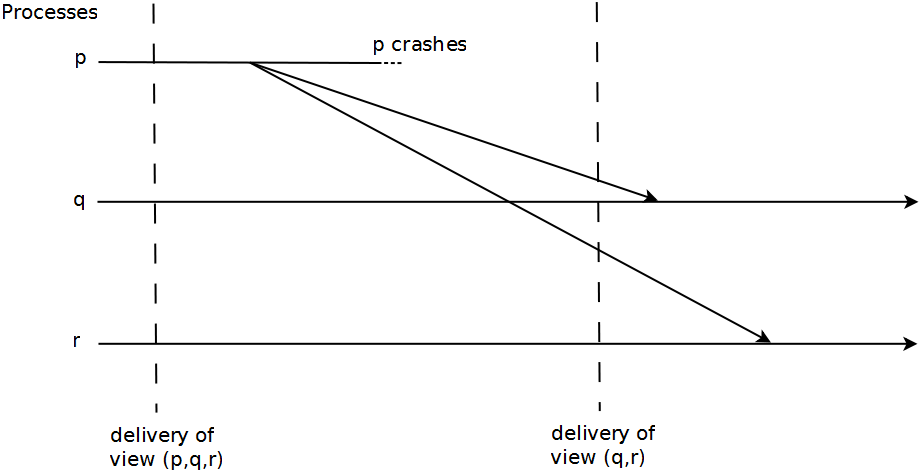
\includegraphics[width=\textwidth]{img/systems-and-architectures/viewsynchronousgroupcommunication_c}
                                        \caption{Disallowed case where the messages are delivered after the delivery of view (q,r) which does not contain the crashed process p.}
                                        \label{figure:viewsynchronousgroupcommunication:c}
        \end{subfigure}
        ~
        \begin{subfigure}[t]{0.4\textwidth}
                                        \centering
                                        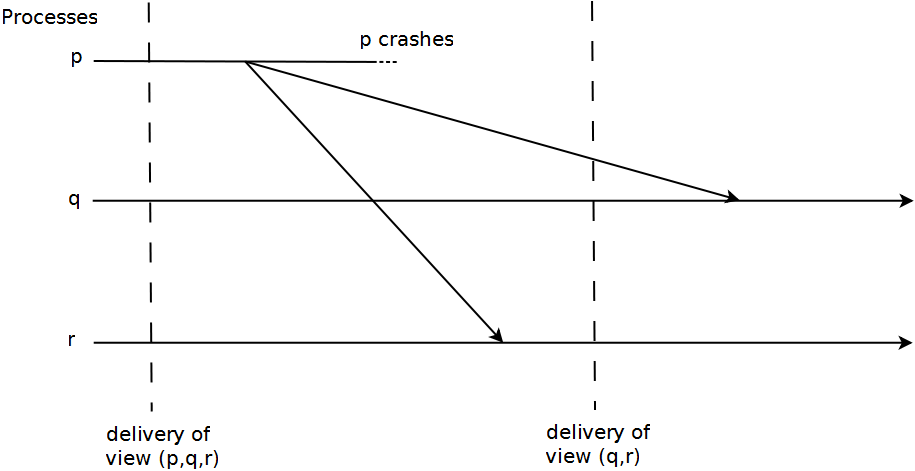
\includegraphics[width=\textwidth]{img/systems-and-architectures/viewsynchronousgroupcommunication_d}
                                        \caption{Disallowed case where the messages are delivered in an incorrect order with regard to view delivery of (q,r).}
                                        \label{figure:viewsynchronousgroupcommunication:d}
        \end{subfigure}
        \caption{A selection of the screens used in the user study with paper prototype.}%
        \label{figure:viewsynchronousgroupcommunication}%
\end{figure}


View-synchronous group communication can be used to perform state transfer from the current group to new members. To ensure that the transferred state is not corrupt, the execution is usually temporary suspended. When the transfer is complete, the coordinator sends a message to the group members to continue.

The goal of group views is to increase fault-tolerance and transparency. As members crash or become unreachable, they are marked "suspicious" and may be excluded from the group by the membership service. This introduces a design challenge, as when excluding processes that are falsely excluded, resources and processing power may be (temporary) lost \cite{Coulouris:2011:DSC:2029110}.

Another design decision has to be made in how to handle network partitions. Two general approaches exist: either the group is reduced, keeping only the primary-partition, or the group is partitionable into subgroups that can continue working independently [1].



\subsection{Fault tolerance}

The goal of fault tolerant systems is to "provide a service that is correct despite up to f process failures" [1]. This can be achieved by replicating data and functionality at replica managers. Correctness of replicated objects is subject to a number of criteria, which can vary in strictness.

\emph{Linearizability} is a strong correctness requirement. Consider a sequence of operation invocations and responses, called a \emph{history}, $o_{2,0}$, $o_{2,1}$, $o_{1,0}$, $o_{2,2}$, $o_{1,1}$, $o_{1,2}$, ..., where \emph{i} represents a client performing an operation \emph{j} for an operation $o_{i,j}$. \textbf{Figure} \ref{figure:linearizability:a} shows an overview of this setup. "A replicated shared object is linearizable if for any execution there is some interleaving of the series of operations issued by all clients that satisfies the following criteria" \cite{Coulouris:2011:DSC:2029110} :
\begin{itemize}
	\item The interleaved sequence of operations meets the specification of a (single) correct copy of the objects.
	\item The order of operations in the interleaving is consistent with the real times at which the operations occurred in the actual execution.
\end{itemize}
\textbf{Figure} \ref{figure:linearizability:b} shows how the operations in the history can be re-ordered. If there exists an ordering for which the previous conditions are met, the system is linearizable. In \textbf{figure} \ref{figure:linearizability:c} the new ordering did not meet the requirement.


\begin{figure}[h]
        \centering
        \begin{subfigure}[t]{0.3\textwidth}
                                        \centering
                                        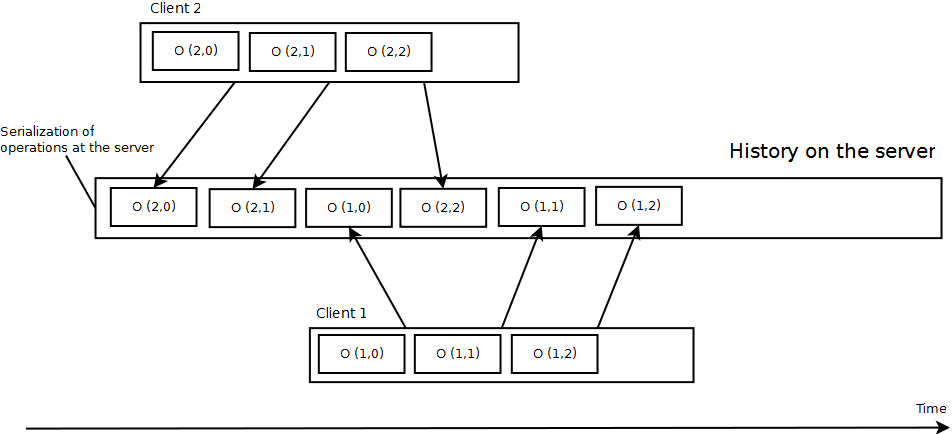
\includegraphics[width=\textwidth]{img/systems-and-architectures/linearizability_1}
                                        \caption{Two clients executing operations on a replicated object managed by a server. The operations are serialized by the server into a certain sequence.}
                                        \label{figure:linearizability:a}
        \end{subfigure}%
        ~
        \begin{subfigure}[t]{0.3\textwidth}
                                        \centering
                                        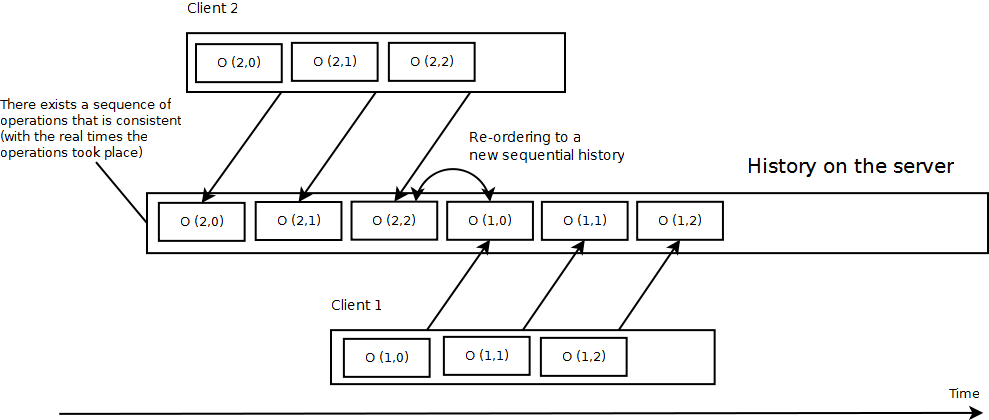
\includegraphics[width=\textwidth]{img/systems-and-architectures/linearizability_2}
                                        \caption{The order of operations can be altered (serializibility) to obtain a new sequence that is consistent with the real times at which the operations occurred in the actual execution.}
                                        \label{figure:linearizability:b}
        \end{subfigure}
        ~
        \begin{subfigure}[t]{0.3\textwidth}
                                        \centering
                                        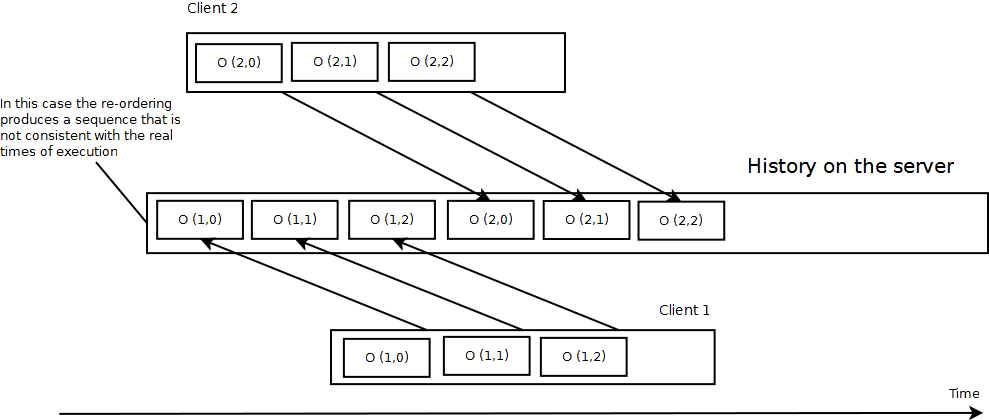
\includegraphics[width=\textwidth]{img/systems-and-architectures/linearizability_3}
                                        \caption{The new sequence that is consistent not with the real times at which the operations occurred in the actual execution.}
                                        \label{figure:linearizability:c}
        \end{subfigure}
        \caption{}
        \label{figure:linearizability}
\end{figure}


\emph{Sequential consistency} is an example of a weak correctness critrium. The requirements for sequential consistency are the following:
\begin{itemize}
	\item The interleaved sequence of operations meets the specification of a (single) correct copy of the objects.
	\item The order of operations in the interleaving is consistent with the program order in which each individual client executed them.
\end{itemize}
As a result, the situation in \textbf{figure} \ref{figure:linearizability:c} is valid under a sequential consistency requirement. The absolute times are not important top obtain sequential consistency, just the order of events corresponding the clients seperately. It should be clear that sequential consistency is a much weaker constraint than linearizability. There may still be inconsistencies in the overal history, despite equential consistency. For example [2] when two clients try to lock an object, one lock will be successful and the other won't. In the case of sequential consistency, it is possible that the negative response is ordered before the successful response, which is not consistent with the sequential definition of the object, i.e. the first one to lock should have gotten a response of success.


\subsubsection{Passive replication}

The model for \emph{passive replication}, the so-called \emph{primary backup model of replication for fault tolerance}, consists out of primary replica manager and a collection of secondary replica managers or "backups". All operations are processed by the primary replica manager and afterwards changes are propagated to the backups. If the primary replica manager should fail, one of the backups is promoted to primary replica manager \cite{Coulouris:2011:DSC:2029110}. \textbf{Figure} \ref{fig:passivereplication} shows an overview of this model.


\begin{figure}[h]
	\begin{center}
		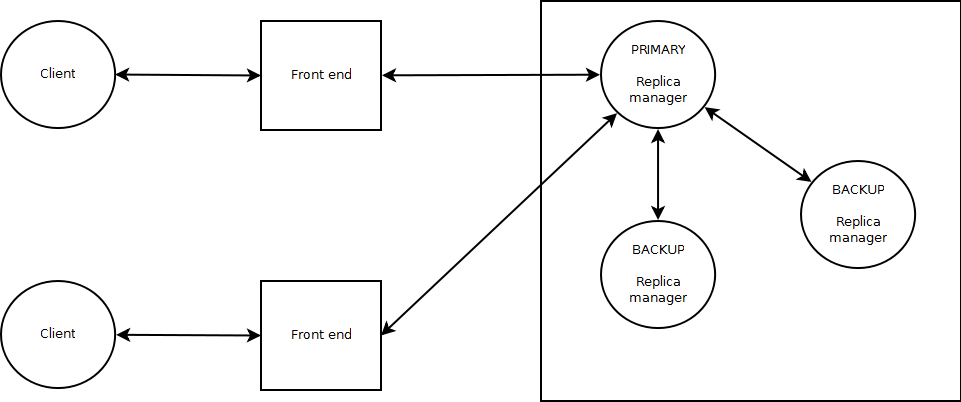
\includegraphics[width=0.7\textwidth]{img/systems-and-architectures/passivereplication}
	\end{center}
	\caption{Passive replication model for fault tolerance.}
	\label{fig:passivereplication}
\end{figure}

The following steps occur when an operation is performed by a client \cite{Coulouris:2011:DSC:2029110}:
\begin{enumerate}
	\item \textbf{Request} : The front end issues the request, containing a unique identifier, to the primary replica manager.
	\item \textbf{Coordination} : The primary takes each request anatomically, in the order in which it receives it. It checks the unique identifier, in case it has already executed the request, and if so, it simply resends the response.
	\item \textbf{Execution} : The primary executes the request and stores the response.
	\item \textbf{Agreement} : If the request is an update, then the primary sends the updated state, the response and the unique identifier to all the backups. The backups send an acknowledgement.
	\item \textbf{Response} : The primary responds to the front end, which hands the response back to the client.
\end{enumerate}

The primary sequences all the operations upon the shared objects, so as long as the primary is correct, the system is linearizable. In the case that the primary fails, however, to ensure linearizability, the primary replica manager has to be replaced by a unique backup, and the remaining replica managers agree which operations had been performed when the replacement primary takes over. This will be the case if the replica managers apply view-synchronous group communication to send updates to the backups \cite{Coulouris:2011:DSC:2029110}.



\subsubsection{Active replication}

In \emph{active replication} the replica managers are state machines with equivalent status and organized as a group. The front end multicasts requests to the group. Within the group each manager processes the requests independently in the same manner and reply individually to the front end \cite{Coulouris:2011:DSC:2029110}. \textbf{Figure} \ref{fig:activereplication} shows the model for active replication.

\begin{figure}[h]
	\begin{center}
		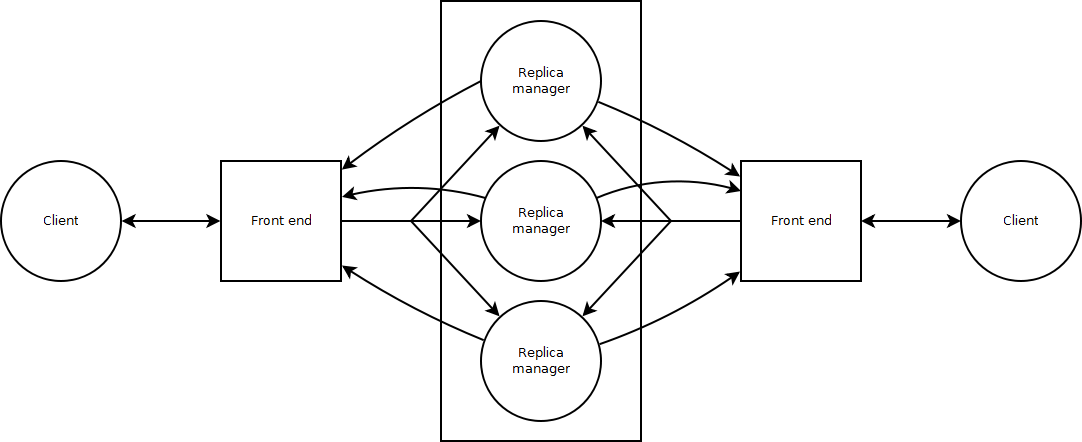
\includegraphics[width=0.7\textwidth]{img/systems-and-architectures/activereplication}
	\end{center}
	\caption{Active replication model for fault tolerance.}
	\label{fig:activereplication}
\end{figure}


The following steps occur when an operation is performed by a client \cite{Coulouris:2011:DSC:2029110}:
\begin{enumerate}
	\item \textbf{Request} : The front end attaches a unique identifier to the request and multicasts it to the group of replica managers, using a totally ordered, reliable multicast primitive. The front end is assumed to fail by crashing at worst.It does not issues the next request until it has received a response.
	\item \textbf{Coordination} : The group communication system delivers the request to every correct replica manager in the same (total) order.
	\item \textbf{Execution} : Every replica manager executes the request. Since they are state machines and since requests are delivered in the same total order, correct replica managers all process the request identically. The response contains the client's unique request identifier.
	\item \textbf{Agreement} : No agreement phase is needed, because of multicast delivery semantics.
	\item \textbf{Response} : Each replica manager sends its response to the front end. The number of replies that the front end collects depends upon the failure assumptions and the multicast algorithm.
\end{enumerate}

The system is sequentially consistent, but does not achieve linearizability since the total ordering is not necessarily the same as the real-time order in which the clients made their requests \cite{Coulouris:2011:DSC:2029110}.

Crashes of replica managers have little impact on the performance in active replication, as the remaining replica managers continue to work as usual. Because the front end can compare the replies it receives, the system is less prone to Bynzantine failures \cite{Coulouris:2011:DSC:2029110}.


\subsubsection{Comparison: active and passive replication}


\begin{table}
	\caption{Comparison between passive and active replication.}
	\label{tab:compare:replication:faulttolerance}
	\begin{tabular}{p{80px} | p{155px} | p{155px}}
															& \textbf{Passive} & \textbf{Active} \\
		\hline
		\textbf{Correctness} 			& Support for linearizability. & Support up to sequential consistency. \\
		\textbf{Fault tolerance} 	& The system requires $f+1$ replica managers to survive up to f process crashes. & For f Byzantine failures, the system requires $2f+1$ replica managers to ensure that the system continues to function correctly. This is because the front collects $f+1$ replies before passing on the results to the client. \\
		\textbf{Efficiency} 			& View-synchronous group communication is required to support linearizability, but introduces a significant overhead. In a variation where read requests are handled by backups to improve performance, the system looses its linearizability property, but maintains sequential consistency. & As managers work independently within te group, crashes have no impact on efficiency. The group communication is relatively cheap as no view-synchronous communication is required. \\
		\hline
	\end{tabular}
\end{table}






%%%%%%%%%%%%%%%%%%%%%%%%%%%%%%%%%%%%%%%%%%%%%%%%%%%%%%%%%%%%%%%%%
\section{Architectures}

\subsection{Client-server}


\subsection{Peer-to-peer}


\subsection{Service-oriented architecture}


\subsection{Cloud computing}

















